\documentclass[10pt]{article}
\usepackage{amsmath}
\usepackage{amssymb}
\usepackage{graphicx}
\usepackage{cite}
\usepackage{color} 

\topmargin 0.0cm
\oddsidemargin 0.5cm
\evensidemargin 0.5cm
\textwidth 16cm 
\textheight 21cm

% Bold the 'Figure #' in the caption and separate it with a period
% Captions will be left justified
\usepackage[labelfont=bf,labelsep=period,justification=raggedright]{caption}

% Use the PLoS provided bibtex style
\bibliographystyle{plos2009}

% Remove brackets from numbering in List of References
\makeatletter
\renewcommand{\@biblabel}[1]{\quad#1.}
\makeatother


% Leave date blank
\date{05/16/2014}

\pagestyle{myheadings}

\begin{document}

% Title must be 150 characters or less
\begin{flushleft}
{\Large
\textbf{Galaxy Zoo: Identifying galaxies}
}
% Insert Author names, affiliations and corresponding author email.
\\
Jeffrey Ning, 
Darshan Hegde 
\\
jkn233@nyu.edu, dh1806@nyu.edu
\end{flushleft}

\section*{Introduction}

<<<<<<< Updated upstream

=======
>>>>>>> Stashed changes
\section*{Problem Definition}

Given an image of a galaxy, we need to predict the probability that it belongs to one of the given morpho- logical categories. The top left part of the poster shows examples from each category. On the left class 1.1 (Smooth Galaxy), in the middle is class 1.2 (Spiral Galaxy) and on the right is class 1.3 ( Star / Artifact).

\section*{Data Description}

The label for each image comes from a collaborative tagging effort by volunteers, in which 40-50 people classified each image as belonging to certain morpho- logical categories. The labels are averaged, so that we have a probability distribution across classes, in- stead of just a single label for each class. The data- set we chose for our project is subset of this, as we only consider 3 categories. We use 30,789 images as a training set and 30789 images as a test set. We use 5 fold cross validation ( CV ) to choose among different features, models and hyper-parameters. Figure \ref{fig:data} shows examples of 3 classes of galaxies.  

\begin{figure}[h]
\begin{center}

\includegraphics[scale=1.35]{images/class_examples.png}
\linebreak
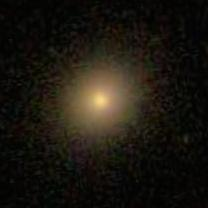
\includegraphics[scale=0.6]{images/Class1_1.jpg}
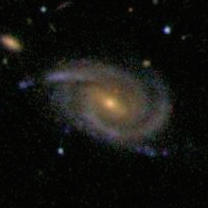
\includegraphics[scale=0.6]{images/Class1_2.jpg}
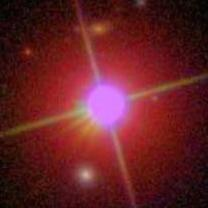
\includegraphics[scale=0.6]{images/Class1_3.jpg}
\caption{Galaxy class examples}
\end{center}
\label{fig:data}
\end{figure}


\section*{Feature Description}

\subsection*{Histogram of Gradients (HoG) Features}
We first convert the image to grayscale. We crop the center $ 208 \times 208 $ pixels and resize it down to $104 \times 104$. We then calculate HoG features as follows. Given an image, we first take a small $k \times k$ patch of image ($8 \times 8$ pixels in our case), and we calculate gradient vectors for each pixel. Then we build a histogram with r bins ( 8 bins in our case), each bin corresponds to ${[(180/r)i, (180/r)(i+1)]} , i=\{0, .. (r-1)\}$. Each bin contains sum of magnitudes of all gradient vectors in that bin. We do this for all patches in the image and concatenate all the histogram vectors. We only consider non overlapping patches, so for $104 \times 104$ image, we have 169 patches by $8 \times 8$ patch size. Our HoG features have dimension of 1352. \ref{fig:hog} shows the HoG calculations on a sample image: 


\begin{figure}[h]
\begin{center}
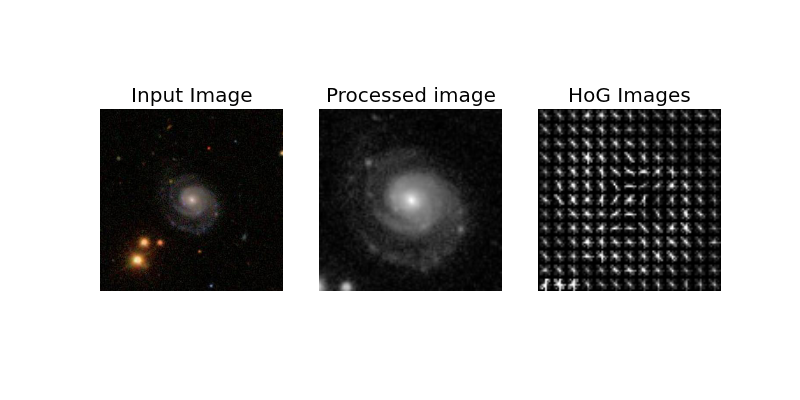
\includegraphics[scale=0.6]{images/HoG_features_noisy.png}
\caption{HoG feature Transformation}
\end{center}
\label{fig:hog}
\end{figure}


\subsection*{Raw Pixel based Features}

Naively, it would seem that using the raw pixels as features, would give us the maximal amount of information possible for our models. However, doing so gave us two major problems. Firstly, our time and space complexity would increase dramatically.

Secondly, we could imagine that it might take more images in our training set to learn accurately. The reason for this could be that that the informative area usually lies in a concentrated subsection of the image and small translation of this informative area could cause large shifts in model prediction.

In order to balance

Our methodology for using raw pixels as features, was to find the center of mass of the image and find the minimum bounding box that surrounds it. We ensured that this bounding box was a square, so that when we resized the image, we would not skew it. Following this we would resize the squre to a (k × k × 3) (the 3 comes from rgb) feature vector. Figure \ref{fig:raw} shows the transformation from original image to final feature.

\begin{figure}[h]
\begin{center}
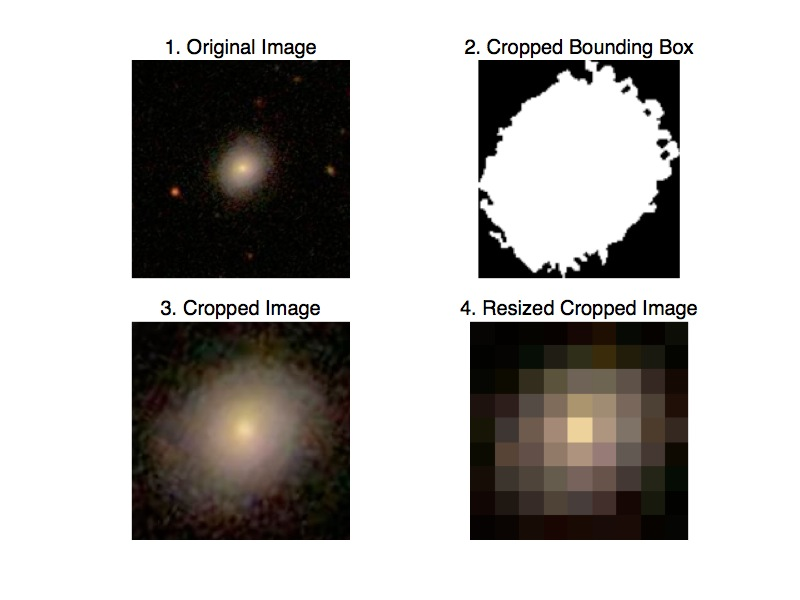
\includegraphics[scale=0.4]{images/hand_engineered_features.jpg}
\caption{Raw pixel based feature transformation}
\end{center}
\label{fig:raw}
\end{figure}

$<explain the chart experiements in detail>$ \ref{fig:raweval} shows the evaluation for different sizes.

\begin{figure}[h]
\begin{center}
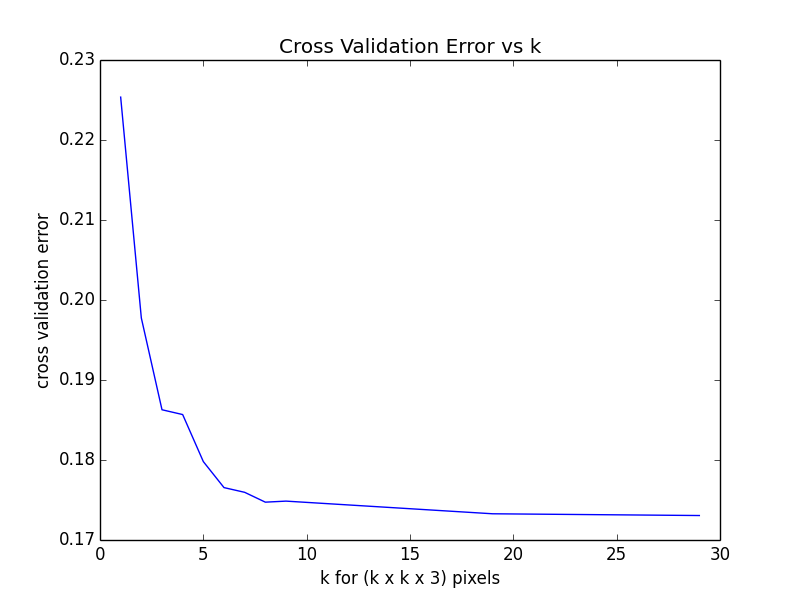
\includegraphics[scale=0.4]{images/find_k_cv.jpg}
\caption{Raw pixel feature performance for different window sizes}
\end{center}
\label{fig:raweval}
\end{figure}

\section*{Model Description}

\subsection*{Decision Tree Regression}
Decision tree regression is a very simple non-linear regression technique. Using training data, we obtain tree structure, which is basically the series of questions about features. Inference involves, running an image through series of yes / questions (In our case, questions corresponds to a pixel and a threshold value for the pixel [Eg: $pixel(22, 23) >= 54$]). After reaching the corresponding leaf in the tree, the probability values for all 3 classes are averaged to get the prediction for that image.   

The training objective is to get leaf nodes such that, training examples which end up in the same leaf node have very close target values. Closeness of target values are measured by mean square error. Mean square error over the entire training set is defined as:

$$MSE = {1 \over n}  \sum_{c \in leaves(T)} \sum_{i \in c} (y_i - m_c)^2$$

where, $m_c =  {1 \over n_c} \sum_{i \in c} y_ic$. $m_c$ is the prediction for that leaf c. We can't do a direct minimization, so we a greedy search. We start by finding the one binary question which minimizes the MSE; this gives us our root node and two child nodes. At each child node, we repeat our initial procedure, asking which question would give us the minimum MSE, given where we already are in the tree. We repeat this recursively. There are several criteria to decide when to stop the recursion. We can set a maximum depth for the tree or minimum samples per leaf or minimum samples a leaf need to have to be considered for splitting. We choose to the last criterion and decide the threshold using cross-validation.

The basic regression-tree-growing algorithm then is as follows:

\begin{itemize}
  \item Start with a single node containing all points. Calculate $m_c$ and MSE.
  \item Search over all binary splits ( pixel and threshold for the pixel ), and find the split that results in minimum MSE, and use the split to create child nodes.
  \item In each child node, consider the node if number of examples are above the threshold. Else, stop splitting that node and consider next child, re-curse \ldots
\end{itemize}

\subsection*{Random Forest Regression} 

Random forest regression, is an ensemble method which fits $n$ number of decision trees and averages their results. While building decision trees, it uses MSE to measure the quality of split and considers only a random subset of $ \log_2(total features)$, to do each split. By considering random subset of features during each split, each decision tree in random forest look very different from each other, which is very desirable. Because, they fit different parts of feature space well.  

\subsection*{Lasso Regression}

Lasso is $L_1$ regularized linear regression. The cost function used is:

$${1 \over (2*n_samp)} \| y -Xw \|^2 + \alpha * \| w \|_1$$

Where y is target $(n\_samp \times 3)$, $X (n\_samp \times n\_feat)$ is input feature matrix and w $(n\_feat \times 3)$ is parameter matrix. The scikits-learn implementation uses coordinate descent to optimize the above cost function. Since lasso uses L1 penalty, one interesting property is that, it tries to find as sparse weight vectors are possible. In our case, since we expect only few pixels to be informative, we use this model. The model is linear, it is not well suitable for vision tasks using very low level features such as HoG, raw pixels. But, it's a good baseline model to compare the results and for doing sanity check of the coding framework, because it's relatively fast to run.

\section*{Evaluation}

We use 2 different measures for evaluation measures. Root Mean Square Error ( RMSE ) and Average KL Divergence.

$$RMSE = {1 \over 3*n} \sum_{i \in \{1, ... N\}} \sum_{j \in \{1, 2, 3\} }{ (y_{ij} - \hat{y_{ij}})^2 }$$

$$Avg D_{KL}(P \| Q)= {1 \over n} \sum_{i \in \{1, ... N\}} \sum_{j \in \{1, 2, 3\} }{ P(i, j) ln{( P(i, j) \over Q(i, j)} ) }$$

We evaluate features by comparing the RMSE and $ Avg D_{KL} $ for Random Forest Regression, with the best hyper-parameter setting, on the validation set. We use 5-fold CV while holding the number of trees in the forest, fixed to 100. Figure \ref{fig:hogdreval} shows the performance of HoG features on decision tree for different setting of minimum samples required to split a node. As seen from the graph, the best performance is achieved at  $ min\_sample\_split = 902$ with $RMSE=0.206203$ and $ Avg D_{KL} = 0.177342 $. Figure \ref{fig:rawdreval} shows Raw feature performance on decision trees for different setting of minimum samples required to split a node. As graph dictates the best performance is achieved at $ min\_sample\_split = $ with $RMSE= $ and $ Avg D_{KL} =  $. The graph indicate classic under-fitting as we increase $ min\_sample\_split $ and over-fitting as decrease $ min\_sample\_split $ beyond the optimal value. Clearly, Raw features do much better in this case. 

To understand why, we plot the feature importance heat-map for both HoG and Raw pixel based features. Feature importance for decision trees are calculated considering number of points, a feature / pixel influences. Higher up the feature / pixel in a decision tree, more number of points it influences and higher is it's feature importance. We use the scikits learn implementation of decision tree regression, which by default calculates this score and precise formula of which is hidden in the code and we did not explore it in detail. For HoG features, we take max over different bins and plot the feature importance for $13 \time 13$ different patches. For raw features, we take max over the channel feature importance for $9 \times 9$ pixels. We look at how many of pixels are active and how they are spatially distributed to understand which part of the images were useful during prediction. Figure \ref{fig:hogdtheat} shows the feature importance heat-map for Hog and Figure \ref{fig:rawdtheat} shows it for raw features. For the decision tree, as seen from the heat-maps, raw pixels are more active and distributed well specially. We believe that, this property is giving the raw feature a slight boost in performance.

\begin{figure}
\begin{center}
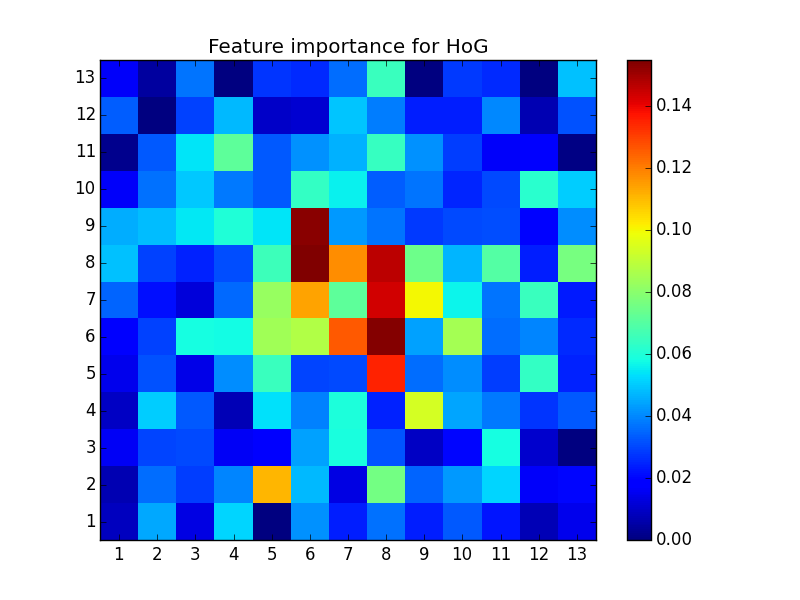
\includegraphics[scale=0.4]{images/HoG_DT_Heatmap.png}
\caption{Feature importance matrix for HoG features}
\label{fig:hogdtheat}
\end{center}
\end{figure}

\begin{figure}
\begin{center}
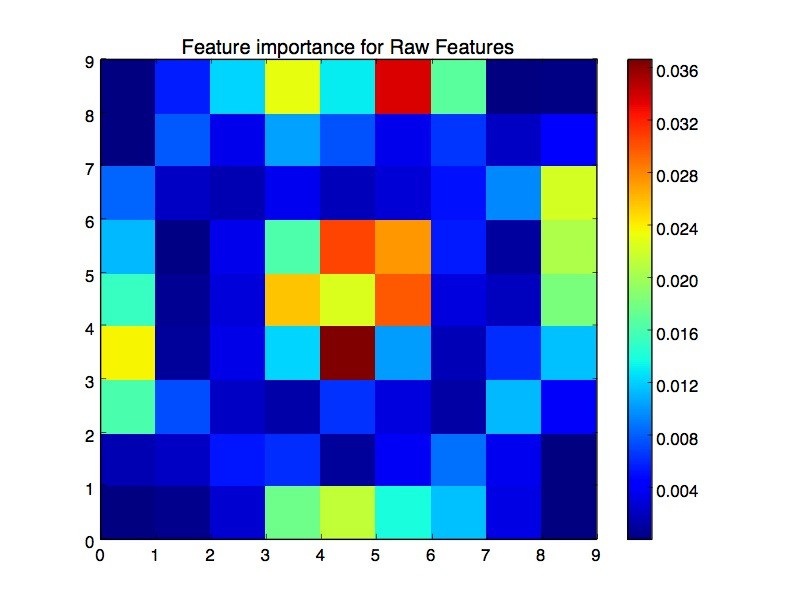
\includegraphics[scale=0.4]{images/Raw_Features_DT_Heatmap.jpg}
\caption{Feature importance matrix for raw features}
\label{fig:rawdtheat}
\end{center}
\end{figure}

\begin{figure}
\begin{center}
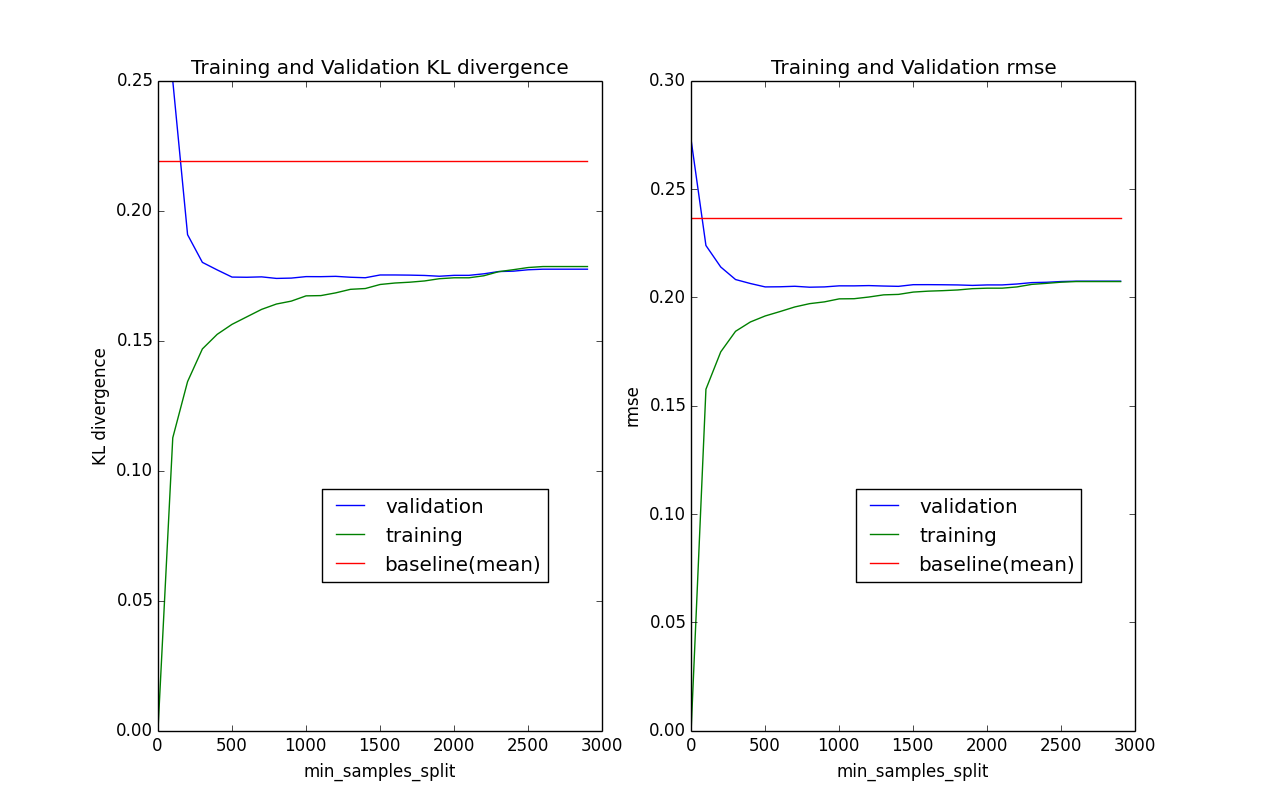
\includegraphics[scale=0.4]{images/HoG_DecisionTreeCV.png}
\caption{HoG feature performance using decision tree regression}
\label{fig:hogdreval}
\end{center}
\end{figure}

\begin{figure}
\begin{center}
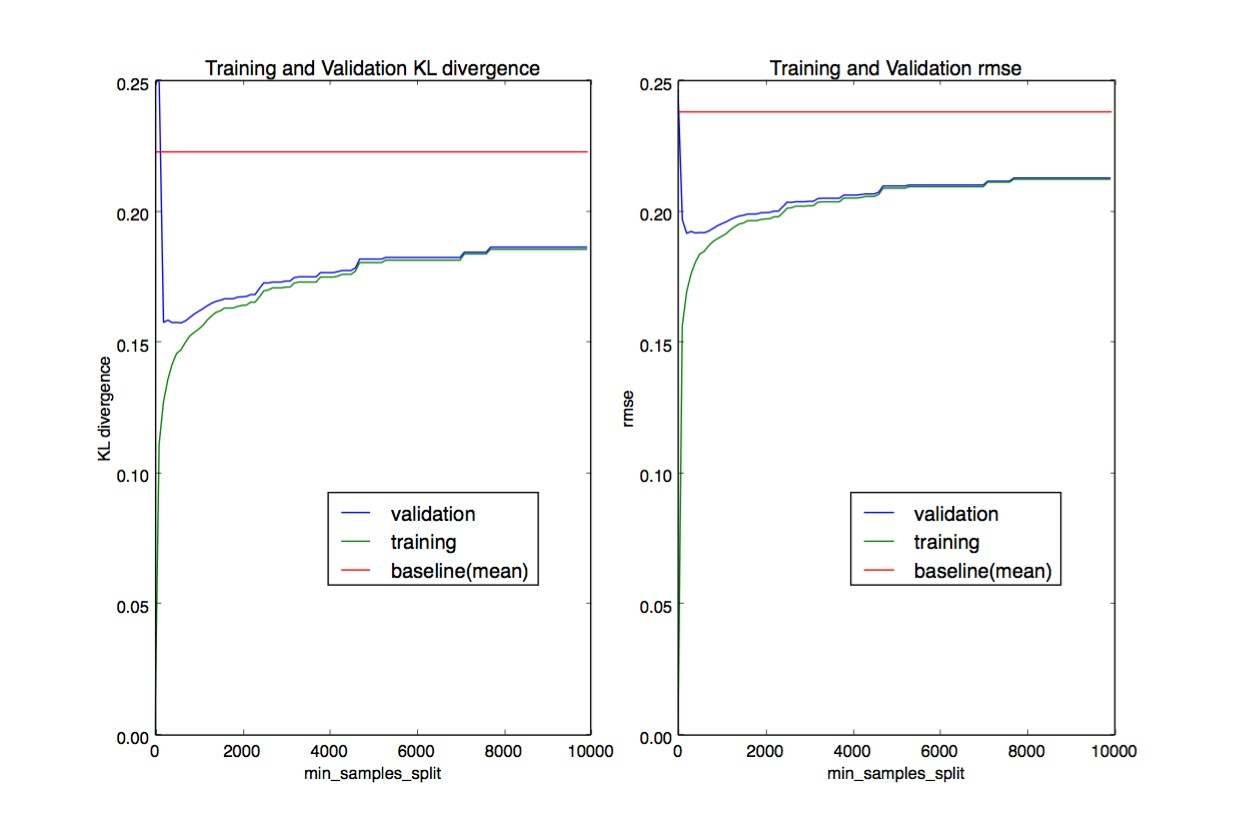
\includegraphics[scale=0.4]{images/Raw_Features_Decision_Tree_min_samples_split.jpg}
\caption{Raw Features Using Decision Trees: Training and Validation Error for min\_samples\_split \\
         Minimum KL-Divergence for Validation: 0.157 min\_samples\_split: 202 \\
         Minimum RMSE for Validation: 0.192: min\_samples\_split: 602}
\label{fig:rawdreval}
\end{center}
\end{figure}


\begin{figure}
\begin{center}
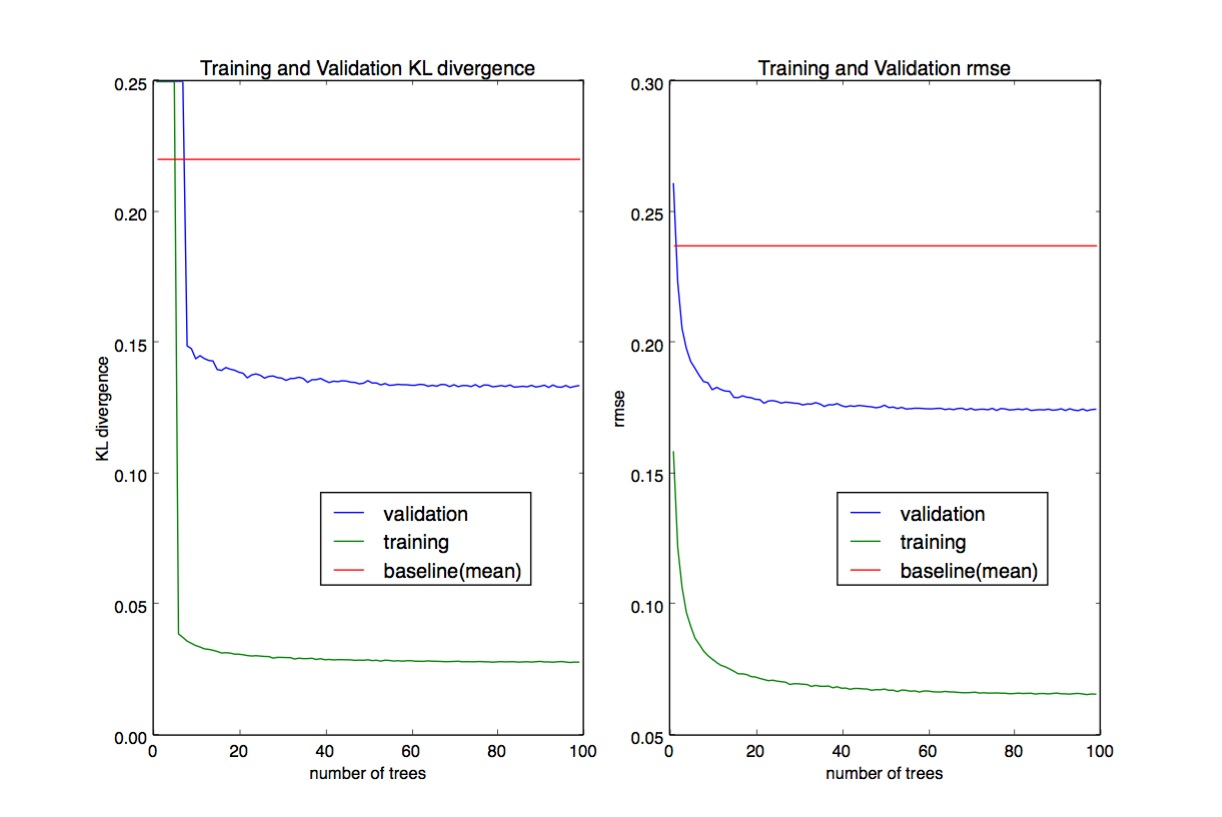
\includegraphics[scale=0.4]{images/Raw_Features_Random_Forest_n_estimators.jpg}
\caption{Raw Features Using Random Forests: Training and Validation Error for n\_estimators \\
         Minimum KL-Divergence for Validation: 0.174 n\_estimators: 97 \\
         Minimum RMSE for Validation: 0.0.133: n\_estimators: 97}
\label{fig:rawdreval}
\end{center}
\end{figure}

\section*{Results}

\section*{Discussion}

\section*{Acknowledgments}

We would like to thank Prof. David Sontag for guiding us through out the project.

\bibliography{template}


\end{document}

